\documentclass[border=3pt,tikz]{standalone}
\usepackage{amsmath}
\usetikzlibrary{arrows.meta}
\usetikzlibrary{calc}
\usetikzlibrary{math}
\usepackage{mathtools}
\begin{document}
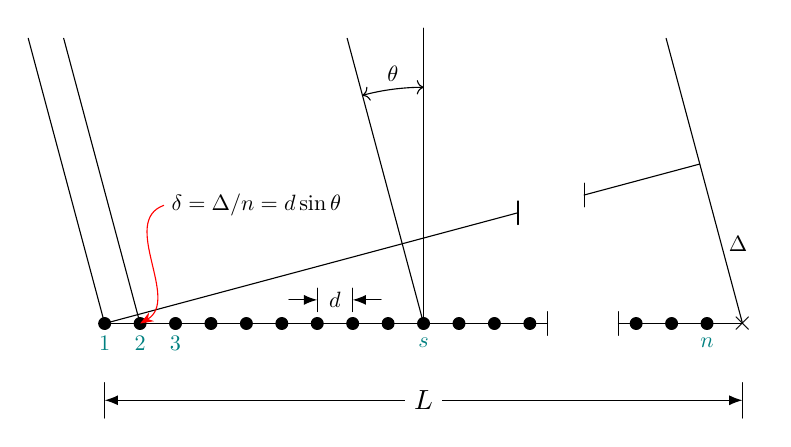
\begin{tikzpicture}[line cap=round, scale=1.5]
    % 관찰자가 움직일때의 도플러 효과
    \def\d{0.3}
    \def\th{15}
    \def\R{3}
    \def\ph{90}
    \def\k{8000}
    \coordinate (P1) at (0, 0);
    \coordinate (P2) at ({\d}, 0);
    \coordinate (P3) at ({2*\d},0);
    \coordinate (P4) at ({3*\d},0);
    \coordinate (S) at ({9*\d}, 0);
    \coordinate (Px) at ({18*\d},0);
    \coordinate (C1) at ({\th}: {12.5*\d*cos(\th)});
    \coordinate (C2) at ({\th}: {14.5*\d*cos(\th)});

    \filldraw[] (P1) circle (0.05) node[yshift=-7, scale=0.8, teal] {$1$};
    \filldraw[] (P2) circle (0.05) node[yshift=-7, scale=0.8, teal] {$2$};
    \filldraw[] (P3) circle (0.05) node[yshift=-7, scale=0.8, teal] {$3$};
    
    
    \foreach \n in {3, ..., 12}{
        \filldraw[] ({\n*\d}, 0) circle (0.05);
    };

    \draw[] (0, 0) -- ({12.5*\d}, 0);
    \draw[] ({12.5*\d}, -0.1) -- ({12.5*\d}, 0.1);
    \draw[] ({14.5*\d}, -0.1) -- ({14.5*\d}, 0.1);
    
    \foreach \n in {15, ..., 17}{
        \filldraw[] ({\n*\d}, 0) circle (0.05);
    };

    \node[yshift=-7, scale=0.8, teal] at (S) {$s$};

    \draw [] (0, -0.5) -- (0, -0.8);
    \draw [] (18*\d, -0.5) -- (18*\d, -0.8);
    \draw [Latex-Latex] (0, -0.65) -- node [ midway,fill=white ] {$L$} (18*\d, -0.65);
    \draw[] ({14.5*\d}, 0) -- ({18*\d}, 0);
    \node [] at ({18*\d}, 0) {$\times$};
    \node[yshift=-7, scale=0.8, teal] at ({17*\d}, 0) {$n$};

    \draw[] ({6*\d}, 0.3) -- ({6*\d}, 0.1);
    \draw[] ({7*\d}, 0.3) -- ({7*\d}, 0.1);
    \draw[-Latex] ({5.2*\d}, 0.2) -- ({6*\d}, 0.2) ;
    \draw[Latex-] ({7*\d}, 0.2) -- ({7.8*\d}, 0.2) ;
    \node[scale=0.8] at ({6.5*\d}, 0.2) {$d$};
    
    \draw [] (P1) -- ++ ({90+\th}:2.5);
    \draw [] (P2) -- ++ ({90+\th}:2.5);
    \draw [] (Px) -- ++ ({90+\th}:2.5);
    
    \draw [] (P1) -- (C1);
    \draw [] ($(C1) + (0, -0.1)$) -- ($(C1) + (0, 0.1)$);
    \draw [] ($(C2) + (0, -0.1)$) -- ($(C2) + (0, 0.1)$);
    \draw [] (C2) -- ({\th}: {18*\d*cos(\th)});
    

    \node [right, scale=0.8] at (0.5, 1) {$\delta = \Delta/n = d \sin \theta$}; 
    \draw[-{Stealth}, red] (0.5, 1)  to [out=2000,in=30,looseness=1] (P2);
    \draw[] (S) --++ (90:2.5);
    \draw[] (S) --++ ({90+\th}:2.5);
    \draw[<->] ($(90:2) + (S)$) arc (90:{90+\th}:2) node[above, midway, scale=0.8] {$\theta$};
    \node[right, scale=0.8] at ($(Px)+({\th+90}:0.7)$) {$\Delta$};
    \end{tikzpicture}
\end{document}
